\documentclass[12pt]{amsart}

\usepackage{luatex85}
\usepackage{tikz}
\usepackage{bbm}
\usetikzlibrary{3d,arrows,calc,positioning,decorations.pathreplacing,matrix} %,arrows.meta}

\usepackage{calligra,mathrsfs}
\usepackage[all]{xy}
\usepackage{float, comment}
\usepackage{mathtools}
\usepackage{amsmath}
\usepackage{amsthm}
\usepackage{amssymb}
\usepackage{amsbsy}
\usepackage{amstext}
\usepackage{amsopn}
%\usepackage{mathrsfs} % allows \mathscr
\usepackage[mathscr]{eucal}
\usepackage{enumerate}
\usepackage{xcolor}
\usepackage{graphicx} % allows \includegraphics{}s
\usepackage{scalerel}
\usepackage{microtype} % improves formattings
\usepackage[margin=1in,marginparwidth=0.8in, marginparsep=0.1in]{geometry}
\renewcommand{\baselinestretch}{1.2} % changes page formatting
\usepackage[pagebackref, bookmarks=true, bookmarksopen=true, bookmarksdepth=3,bookmarksopenlevel=2, colorlinks=true, linkcolor=blue, citecolor=blue, filecolor=blue, menucolor=blue, urlcolor=blue]{hyperref}
% \usepackage{newtxtext} % improves font appearance
\usepackage{tikz}
\usepackage{bbm}
\usepackage[all]{xy}
\usetikzlibrary{arrows,calc,positioning,decorations.pathreplacing} %,arrows.meta}

\numberwithin{equation}{section}
\newtheorem{Theorem}[equation]{Theorem}
\newtheorem{Proposition}[equation]{Proposition} 
\newtheorem{Lemma}[equation]{Lemma}
\newtheorem{Open}[equation]{Open Question}
\newtheorem{Corollary}[equation]{Corollary}
\newtheorem{Conjecture}[equation]{Conjecture}
\newtheorem{Specialthm}{Theorem}
\newtheorem{Question}{Question}

\theoremstyle{definition}
\newtheorem{Remark}[equation]{Remark}
\newtheorem{Example}[equation]{Example}
\newtheorem{Definition}[equation]{Definition}

\numberwithin{figure}{section}

\def\la{\langle}
\def\ra{\rangle}
\def\ttimes{\widetilde{\times}}
\def\tbox{\widetilde{\boxtimes}}
\def\bbox{{\boxtimes}}
\def\O{\mathcal{O}}
\def\K{\mathcal{K}}
\def\bG{\mathbb{G}}
\newcommand{\gr}{\mathrm{gr}}
\newcommand{\mb}[1]{\mathbf{#1}}
\newcommand{\fsl}{\mathfrak{sl}}
\newcommand{\fg}{\mathfrak{g}}
\newcommand{\fn}{\mathfrak{n}}
\newcommand{\bk}{{\mathbbm k}}
\newcommand{\A}{\mathbb{A}}
\newcommand{\C}{\mathbb{C}}
\newcommand{\D}{\mathbb{D}}
\newcommand{\E}{\mathbb{E}}
\newcommand{\G}{\mathbb{G}}
\newcommand{\bN}{\mathbb{N}}
\renewcommand{\P}{\mathbb{P}}
\newcommand{\Q}{\mathbb{Q}}
\newcommand{\Z}{\mathbb{Z}}
\newcommand{\bfC}{{\mathbf{C}}}
\newcommand{\bfD}{{\mathbf{D}}}
\newcommand{\bfI}{{\mathbf{I}}}
\newcommand{\cA}{\mathcal{A}}
\newcommand{\cB}{\mathcal{B}}
\newcommand{\cC}{\mathcal{C}}
\newcommand{\cD}{\mathcal{D}}
\newcommand{\cE}{\mathcal{E}}
\newcommand{\cF}{\mathcal{F}}
\newcommand{\cG}{\mathcal{G}}
\newcommand{\cH}{\mathcal{H}}
\newcommand{\cK}{\mathcal{K}}
\newcommand{\cL}{\mathcal{L}}
\newcommand{\cM}{\mathcal{M}}
\newcommand{\cN}{\mathcal{N}}
\newcommand{\cO}{\mathcal{O}}
\newcommand{\cP}{\mathcal{P}}
\newcommand{\cQ}{\mathcal{Q}}
\newcommand{\cR}{\mathcal{R}}
\newcommand{\cS}{\mathcal{S}}
\newcommand{\cT}{\mathcal{T}}
\newcommand{\cU}{\mathcal{U}}
\newcommand{\cV}{\mathcal{V}}
\newcommand{\cW}{\mathcal{W}}
\newcommand{\cX}{\mathcal{X}}
\newcommand{\cY}{\mathcal{Y}}
\newcommand{\sW}{\mathscr{W}}
\newcommand{\sX}{\mathscr{X}}
\newcommand{\sY}{\mathscr{Y}}
\newcommand{\sZ}{\mathscr{Z}}

\newcommand{\hs}{\heartsuit}
\newcommand{\bul}{\bullet}
\newcommand{\ga}{\gamma}
\newcommand{\al}{\alpha}
\newcommand{\be}{\beta}

%Commands for Lecture 14
\newcommand{\on}[1]{\operatorname{#1}}
\newcommand{\TeL}{\on{TL}}
\newcommand{\Rcheck}{\breve{R}}
\usepackage{tikzit}
\input{tikzit_styles.tikzstyles}


%% code from mathabx.sty and mathabx.dcl
\DeclareFontFamily{U}{mathx}{\hyphenchar\font45}
\DeclareFontShape{U}{mathx}{m}{n}{
	<5> <6> <7> <8> <9> <10>
	<10.95> <12> <14.4> <17.28> <20.74> <24.88>
	mathx10
}{}
\DeclareSymbolFont{mathx}{U}{mathx}{m}{n}
\DeclareFontSubstitution{U}{mathx}{m}{n}
\DeclareMathAccent{\widecheck}{0}{mathx}{"71}
\DeclareMathSymbol{\shortminus}{\mathbin}{AMSa}{"39}

\DeclareRobustCommand{\SkipTocEntry}[5]{}

\newcommand{\arrtip}{latex'}

\begin{document}
\title{Notes on Schubert Calculus and Quantum Integrability}

\begin{abstract}
\end{abstract}

\maketitle

\setcounter{tocdepth}{1}

\tableofcontents

\section{Introduction}

\thispagestyle{empty}

Here is a template for a simple commutative diagram in tikz:
\begin{equation*}
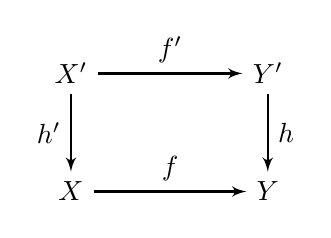
\begin{tikzpicture}
[baseline=(current  bounding  box.center),thick,>=\arrtip]
\node (a) at (0,0) {$X'$};
\node (b) at (2.5,0) {$Y'$};
\node (c) at (0,-1.5) {$X$};
\node (d) at (2.5,-1.5) {$Y$};
\draw[->] (a) to node[above] {$f' $} (b);
\draw[->] (b) to node[right] {$h $} (d);
\draw[->] (a) to node[left] {$h' $}(c);
\draw[->] (c) to node[above] {$f $} (d);
\end{tikzpicture}
\end{equation*}

Here is a template for an elaborate commutative diagram in tikz:
\begin{equation*}
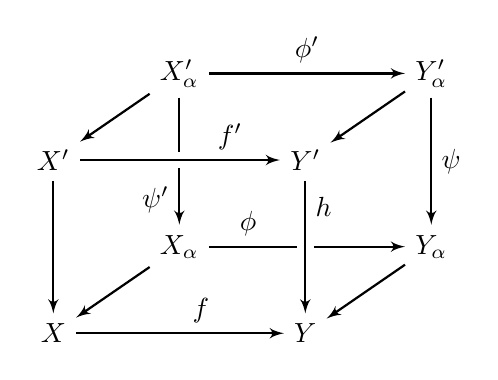
\begin{tikzpicture}[baseline=(current  bounding  box.center),thick,>=\arrtip]
\newcommand*{\ha}{1.6}; \newcommand*{\hb}{1.6}; \newcommand*{\hc}{1.6};
\newcommand*{\va}{-1.1}; \newcommand*{\vb}{-1.1}; \newcommand*{\vc}{-1.1};
\node (ab) at (\ha,0) {$X_\al'$};
\node (ad) at (\ha+\hb+\hc,0) {$Y_\al'$};
\node (ba) at (0,\va) {$X'$};
\node (bc) at (\ha+\hb,\va) {$Y'$};
\node (cb) at (\ha,\va+\vb) {$X_\al$};
\node (cd) at (\ha+\hb+\hc,\va+\vb) {$Y_\al$};
\node (da) at (0,\va+\vb+\vc) {$X$};
\node (dc) at (\ha+\hb,\va+\vb+\vc) {$Y$};
\draw[->] (ab) to node[above] {$\phi' $} (ad);
\draw[->] (ab) to node[above] {$ $} (ba);
\draw[->] (ab) to node[left,pos=.8] {$\psi' $} (cb);
\draw[->] (ad) to node[above] {$ $} (bc);
\draw[->] (ad) to node[right] {$\psi $} (cd);
\draw[->] (ba) to node[above] {$ $} (da);
\draw[->] (cb) to node[above,pos=.2] {$\phi $} (cd);
\draw[->] (cb) to node[above] {$ $} (da);
\draw[->] (cd) to node[above] {$ $} (dc);
\draw[->] (da) to node[above,pos=.6] {$f $} (dc);

\draw[-,line width=6pt,draw=white] (ba) to  (bc);
\draw[->] (ba) to node[above,pos=.75] {$f' $} (bc);
\draw[-,line width=6pt,draw=white] (bc) to  (dc);
\draw[->] (bc) to node[right,pos=.2] {$h $} (dc);
\end{tikzpicture}
\end{equation*}

\section{Lecture 1 (Allen Knutson)}

\section{Lecture 2 (Allen Knutson)}

\section{Lecture 3 (Paul Zinn-Justin)}

\section{Lecture 4 (Paul Zinn-Justin)}

\section{Lecture 5 (Allen Knutson)}

\section{Lecture 6 (Allen Knutson)}

\section{Lecture 7 (Paul Zinn-Justin)}

\section{Lecture 8 (Paul Zinn-Justin)}

\section{Lecture 9 (Allen Knutson)}

\section{Lecture 10 (Allen Knutson)}

\section{Lecture 11 (Paul Zinn-Justin)}

\section{Lecture 12 (Paul Zinn-Justin)}

\section{Lecture 13 (Allen Knutson)}

\section{Lecture 14 (Paul Zinn-Justin)}

\subsection{Basic Definitions}

\begin{Definition}[Temperley-Lieb Algebra]
	Let $\tau$ be a complex number. The Temperley-Lieb Algebra $\TeL_n(\tau)$ is generated by an identity $1$ and generators $e_1, \ldots e_{n-1}$ satisfying the relations
	\begin{itemize}
		\item $e_i^2 = \tau e_i$
		\item $e_i e_{i+1} e_i = e_i$
		\item $e_i e_j = e_j e_i, |i-j|>1$
	\end{itemize}
\end{Definition}

We can give a pictorial description of this algebra: we regard each generator $e_i$ as corresponding to a diagram
\ctikzfig{TLfig1}
and regard $\tau$ as corresponding to the ``fugacity of a bubble." We then multiply by composing vertically (with the rightmost element at the top), and ``popping" bubbles to obtain a factor of $\tau$:
\ctikzfig{TLfig2}

\begin{Example}[$\TeL_3(\tau)$]
	When $n=3$, we have generators $1 = $ \tikzfig{TL3gen1}, $e_1 = $ \tikzfig{TL3gene1}, and $e_2 = $ \tikzfig{TL3gene2}. We also obtain
	\[e_1 e_2 = \tikzfig{TL3e1e2}\]
	and 
	\[e_2 e_1 = \tikzfig{TL3e2e1},\]
	so that $\TeL_3(\tau)$ is $5$-dimensional.
\end{Example}



\begin{Proposition}
	The dimension of $\TeL_n$ is
	\[\dim \TeL_n = C_n = \frac{(2n)!}{n!(n+1)!},\]
	the $n$th Catalan number.
\end{Proposition}

\subsection{Temperley-Lieb Algebras and the Yang-Baxter Equation} We can reinterpret the Yang-Baxter equation through the lens of Temperley-Lieb algebras. Let $\tau = -(q+q^{-1}), a(u) = qu-q^{-1}u^{-1},$ and $b(u) = u-u^{-1}.$ We can then regard $\Rcheck_i$ as an element of the algebra obtained by adding $u^\pm$ and $v^\pm$ to $\TeL_n(\tau)$:
\[\Rcheck_i(u) = a(u) 1 + b(u) e_i \in \TeL_n(\tau)[u^{\pm}, v^{\pm}].\]
One can check that the equation
\[\Rcheck_i(u) \Rcheck_{i+1}(uv) \Rcheck_i(v) = \Rcheck_{i+1}(v) \Rcheck_{i}(uv) \Rcheck_{i+1}(u)\]
holds; we may thus interpret the Yang-Baxter equation as an identity in $\TeL_n(\tau)[u^{\pm}, v^{\pm}].$

Via this identification, we can regard systems satisfying the Yang-Baxter equation as representations of this algebra $\TeL_n(-(q+q^{-1}))[u^{\pm}, v^{\pm}].$ We may obtain one such representation via the map 
\[\phi: \TeL_n(-(q+q^{-1})) \rightarrow \on{End}((\bfC^2)^{\otimes n})\]
sending
\[e_i \mapsto I \otimes I \otimes \ldots \otimes  I \otimes 
\begin{bmatrix}
	0 & 0 & 0 & 0\\
	0 & -q^{-1} & 1 & 0\\
	0 & 1 & -q & 0\\
	0 & 0 & 0 & 0
\end{bmatrix} \otimes I \otimes \ldots \otimes I,\]
where the matrix is located in the $i$ and $i+1$ coordinates. 

One can check that this map respects the Temperley-Lieb relations, and that it induces a representation $\rho: \TeL_n(-(q+q^{-1}))[u^{\pm}, v^{\pm}] \rightarrow \on{End}((\bfC^2)^{\otimes n})$ sending
\[\Rcheck_i(u) \mapsto I \otimes \ldots \otimes  I \otimes 
\begin{bmatrix}
	qu-q^{-1}u^{-1} & 0 & 0 & 0\\
	0 & u(q-q^{-1}) & u-u^{-1} & 0\\
	0 & u-u^{-1} & u^{-1}(q-q^{-1})& 0\\
	0 & 0 & 0 & qu-q^{-1}u^{-1}
\end{bmatrix} \otimes I \otimes \ldots \otimes I\]

\subsection{Loop Models}

\section{Lecture 15 (Allen Knutson)}

\section{Lecture 16 (Allen Knutson)}

\section{Lecture 17 (Paul Zinn-Justin)}

\section{Lecture 18 (Paul Zinn-Justin)}

\end{document}
